\documentclass[12pt,a4paper]{article}
\usepackage{graphicx, booktabs, siunitx, amsmath, geometry, float}
\usepackage{subcaption}
\geometry{margin=2.5cm}
\title{Magneto-Optics}
\author{Gregorio Jaca U8L9B9, Peter Tallosy K14WR1}
\date{\today}

\begin{document}
\maketitle

% Abstract
\begin{abstract}

    Sensitive light polarization allows us to characterize the optical properties of different samples.
    We measured the optical retardation of a voltage controlled liquid crystal (LC) cell. We built a setup which allows us to measure the linear dichroism in hemozoid in suspension, a malaria indicator. Using samples of known concentration, we constructed a calibration curve which allows us to quantify the concentration of an unknown sample.

\end{abstract}

% Introduction
\section{Introduction}

Molecules with anisotropic shapes can have anisotropic orientation-dependent optical effects individually. In most cases, aggregates of randomly oriented molecules have no net anisotropic effect. Liquid crystal (LC) phases at the boundary of a liquid and a solid crystal with an ordered orientation, which can controlled by an electric field. Taking advantage of this property, we use a LC cell with a voltage controlled waveplate which generates the alternating electric field, which acts as a voltage-controlled waveplate.

\section{Theoretical Background}
Light, as an electromagnetic wave, possesses a property known as polarization, which describes the orientation of its oscillating electric field vector \( \mathbf{E} \). In the context of transverse electromagnetic radiation, this orientation can be effectively represented by a 2D vector known as the Jones vector:
\begin{equation*}
\mathbf{E} = \begin{pmatrix} E_{0x}e^{i\delta_x} \\ E_{0y}e^{i\delta_y} \end{pmatrix}
\end{equation*}
where \( E_{0x} \) and \( E_{0y} \) are the amplitudes, and \( \delta_x \) and \( \delta_y \) are the phases of the electric field components along two orthogonal transverse directions. Optical elements can linearly transform the incoming polarization state to an outgoing state, a process described by Jones matrices. For an ideal linear polarizer, which transmits only the electric field component parallel to its transmission axis, the transmitted intensity \( I \) of a linearly polarized light beam follows Malus' Law:
\begin{equation*}
I \propto I_0 \cos^2\varphi
\end{equation*}
Here, \( I_0 \) is the initial intensity and \( \varphi \) is the angle between the light's polarization axis and the polarizer's transmission axis. The quality of a polarizer is quantified by its extinction ratio, defined as the ratio of minimum to maximum transmitted intensity, \( I_\perp / I_\parallel \), where \( I_\perp \) is the intensity when polarizers are crossed, and \( I_\parallel \) is the intensity when they are parallel.

\section{Experimental Setup}
The experimental setup comprised a laser diode as the light source. The emitted light was directed through a series of optical components, including polarizers, a liquid crystal (LC) cell, and detectors. A signal generator was utilized to apply controlled voltages to the LC cell, enabling precise modulation of its optical properties. Measurements of light intensity were conducted using a detector, with data acquisition and analysis facilitated by a lock-in amplifier for enhanced signal-to-noise ratio in specific tasks. Angular adjustments of optical components were performed manually, and efforts were made to mitigate the influence of ambient light.

\section{Results and Discussion}

\subsection{Error Analysis}
Throughout the experimental procedures, several sources of error were identified that could influence the precision and accuracy of the measurements. These include, but are not limited to, fluctuations in ambient light, which were partially mitigated by establishing a baseline, but could not be entirely eliminated. Manual angular adjustments of optical components introduced uncertainties, estimated to be approximately \( \pm 3^\circ \), potentially leading to discrepancies in the measured angular dependencies. Similarly, voltage measurements exhibited an uncertainty of approximately \( \pm 5 \text{ mV} \). Misalignment of the optical axis and potential inherent imperfections in the polarizing components also contributed to deviations from ideal theoretical behaviors, particularly affecting the measured extinction ratio. These factors collectively suggest that while the observed phenomena align with theoretical predictions, quantitative measurements should be interpreted with consideration of these inherent experimental uncertainties.

\subsection{Basic characterization of film polarizers}

% TASK 1

We measured the analyzer orientation dependence of the intensity. Initial measurements considered the room background lighting, establishing a baseline. The data demonstrates a \( I \sim \cos^2\varphi \) dependency of the light intensity with respect to the polarizer angle, consistent with Malus' Law. The extinction ratio, \( \text{extinction\_ratio} = \frac{\text{min}(V)}{\text{max}(V)} \), quantifies the quality of a polarizer; a smaller value indicates higher quality. From our measurements, with a minimum recorded voltage of 66 mV and a maximum of 5.8185 V (after accounting for a background offset of 65 mV, where raw max was 5.8185V and raw min was 72mV, so (72-65)/(5818.5-65)=0.0012) we calculated an extinction ratio of 0.0012. This value confirms the reasonable performance of the polarizers utilized. This characterization also allowed for the determination of the light source's polarization direction and the subsequent calibration of the experimental setup.

\begin{figure} [H]
    \centering
    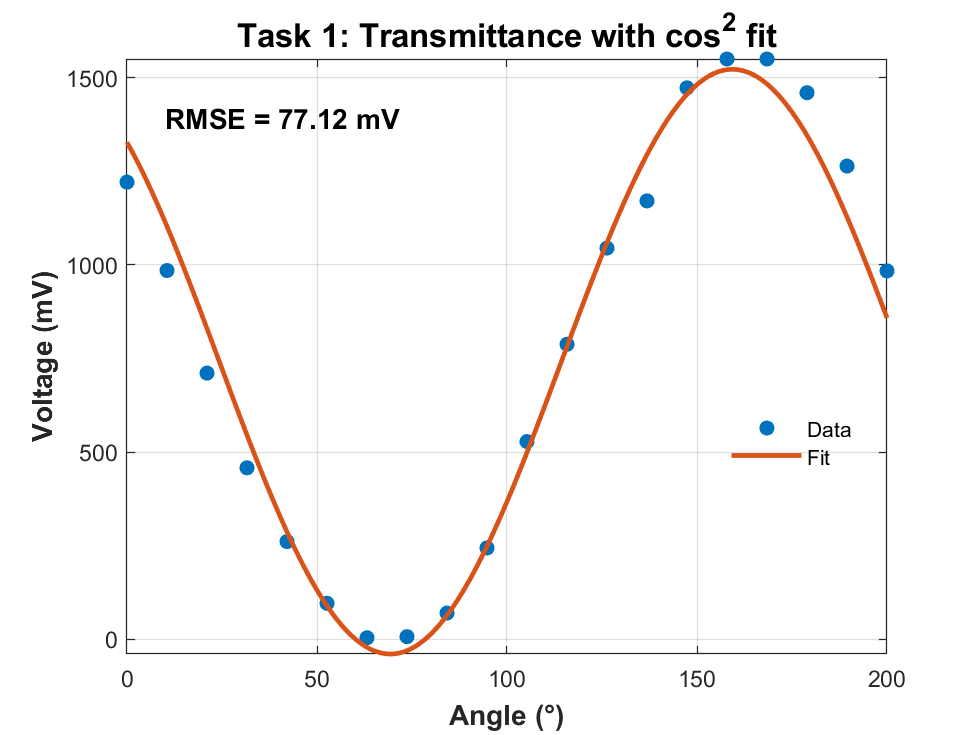
\includegraphics[width=0.6\linewidth]{figs/task1_transmittance_with_cos_squared_fit.png}
    \caption{Light intensity dependency on analyzer orientation.}
    \label{fig:t1}
\end{figure}

The data shows a $I \sim \cos^2\varphi$ dependency of the light intensity with the polarizer angle. The extinction ratio $= \frac{I_\perp}{I_\parallel}$ quantifies the quality of a polarizer, with a smaller value indicating a higher quality, was calculated and we obtained a value of 0.0026. This measurement allowed us to determine the polarization direction of the light source and calibrate our setup.

\subsection{Liquid crystal cell}
The experimental setup for characterizing the liquid crystal (LC) cell involved placing it between two orthogonal linear polarizers. In the absence of the LC cell, minimal light would reach the detector due to the crossed polarizers. However, when the LC cell is positioned at a \( 45^\circ \) angle, it is expected to circularly polarize the incident light. We empirically determined this optimal angle by rotating the LC cell until a maximum intensity was observed at the detector, which occurred at approximately \( 50^\circ \). Ideally, circularly polarized light should exhibit no angular dependence on a subsequent linear analyzer. While the polar plot (Fig. \ref{fig:t2b}) was expected to be circular, the measured angle range was less than \( 360^\circ \), resulting in an incomplete plot. A subtle angular dependency was observed (Fig. \ref{fig:t2a}), reminiscent of the behavior seen in the basic polarizer characterization (Fig. \ref{fig:t1}). This suggests that a minor component of the light was not perfectly circularly polarized and retained some linear polarization, which was subsequently modulated by the analyzer's orientation. The constant, angle-independent component of the signal is attributed to the circularly polarized light, which remains unaffected by the linear analyzer's orientation.

\begin{figure}[H]
    \centering
    \begin{subfigure}[b]{0.48\linewidth}
        \centering
        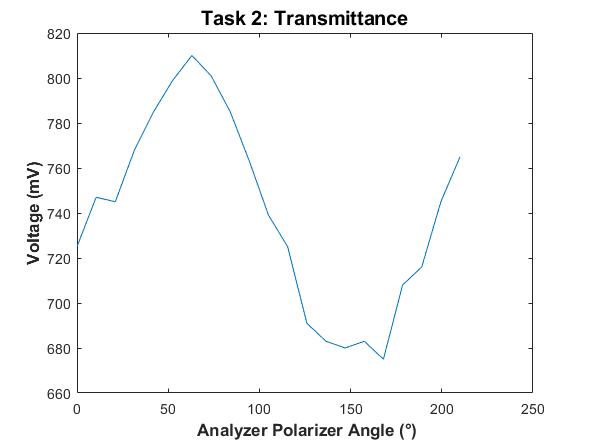
\includegraphics[width=\linewidth]{figs/task2_transmittance.png}
        \caption{Transmittance vs analyzer angle}
        \label{fig:t2a}
    \end{subfigure}\hfill
    \begin{subfigure}[b]{0.48\linewidth}
        \centering
        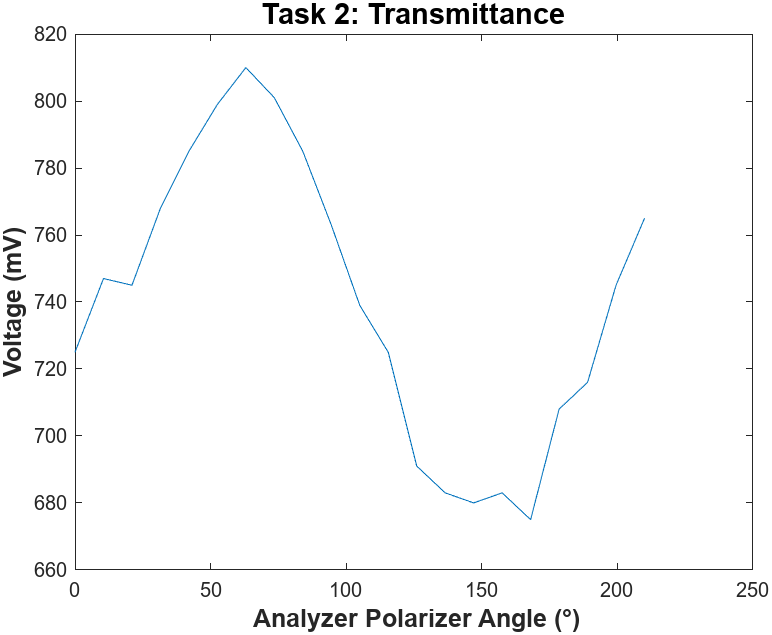
\includegraphics[width=\linewidth]{figs/task2_polar.png}
        \caption{Polar plot of measured intensity}
        \label{fig:t2b}
    \end{subfigure}

    \caption{Left: Light intensity dependency on analyzer orientation. Right: Polar plot of the light intensity as a function of the analyzer orientation. A circular plot indicates an orientation-independent signal. Our measured angle range was unfortunately less than 360°, which prevents a closed polar plot.}
    \label{fig:t2}
\end{figure}

 The small angular dependency resembles the one observed previously (see Fig. \ref{fig:t1}). This suggests that a small component of the light did not get circularly polarized, but rather remained linearly polarized, and it was this component that gets filtered by the analyzer based on its orientation.
 The constant (angle independent) intensity component of the measured signal represent the circularly polarized component of the light, which is not affected by the orientation of the linear analyzer polarizer.
% circular plot


% TASK 3 AND 4
For tasks 3 and 4, a 2 kHz rectangular signal was synthesized and applied to the LC cell. This induced an electric field that caused some liquid crystal molecules to align with the field direction, thereby creating a birefringent cell. This birefringence introduces a phase shift in the passing light, particularly when the LC cell is rotated \( 45^\circ \) with respect to the polarizer. We systematically measured the voltage dependency of the transmitted light intensity under both parallel and orthogonal linear polarizer and analyzer configurations. The relationship between the transmittance and the retardation \( \delta \) when the LC cell is rotated by \( 45^\circ \) is given by:
\begin{align*}
T_\parallel &= \cos^2\!\left(\frac{\delta}{2}\right),\\
T_\perp      &= \sin^2\!\left(\frac{\delta}{2}\right).
\end{align*}
Based on these relationships, \( \delta \) was calculated as a function of the applied voltage amplitude, revealing a strongly non-linear relationship (Fig. \ref{fig:t3_4_delta}). This non-linear response highlights the complex electro-optical properties of the liquid crystal material and its sensitivity to the applied electric field.

\begin{figure}[H]
    \centering
    \begin{subfigure}[b]{0.48\linewidth}
        \centering
        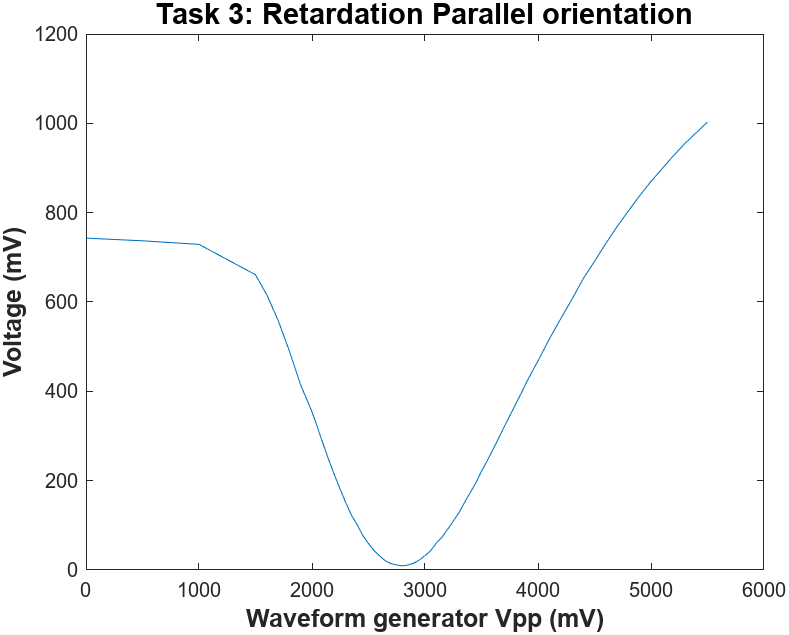
\includegraphics[width=\linewidth]{figs/task3_transmittance.png}
        \caption{Parallel configuration}
        \label{fig:t3}
    \end{subfigure}\hfill
    \begin{subfigure}[b]{0.48\linewidth}
        \centering
        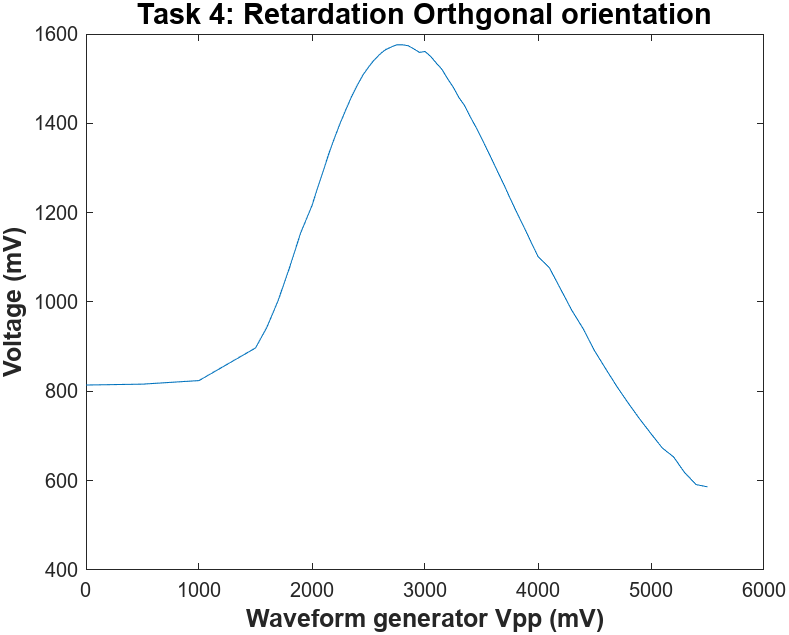
\includegraphics[width=\linewidth]{figs/task4_transmittance.png}
        \caption{Orthogonal configuration}
        \label{fig:t4}
    \end{subfigure}

    \caption{Light intensity as a function of the amplitude of the rectangular AC applied voltage. Left: parallel configuration. Right: orthogonal configuration.}
    \label{fig:t3_4}
\end{figure}

%LLM-COMMENT: commit: place Task 3 and Task 4 plots side-by-side with subcaptions

The relationship between the transmittance and the retardation $\delta$ when the LC cell is rotated by 45° can be expressed as:
% \[
% T_\parallel = \cos^2($delta$/2)
% T_\perp = \sin^2($delta$/2)
% \]
% \[
% T_\parallel = \cos^2\!\left(\frac{\delta}{2}\right), \qquad
% T_\perp = \sin^2\!\left(\frac{\delta}{2}\right)
% \]
\begin{align*}
T_\parallel &= \cos^2\!\left(\frac{\delta}{2}\right),\\
T_\perp      &= \sin^2\!\left(\frac{\delta}{2}\right).
\end{align*}
% G: XXX check

Based on this, we can calculate $\delta$ as a function of the applied voltage amplitude, which shows a strongly non-linear relationship.

\begin{figure} [H]
    \centering
    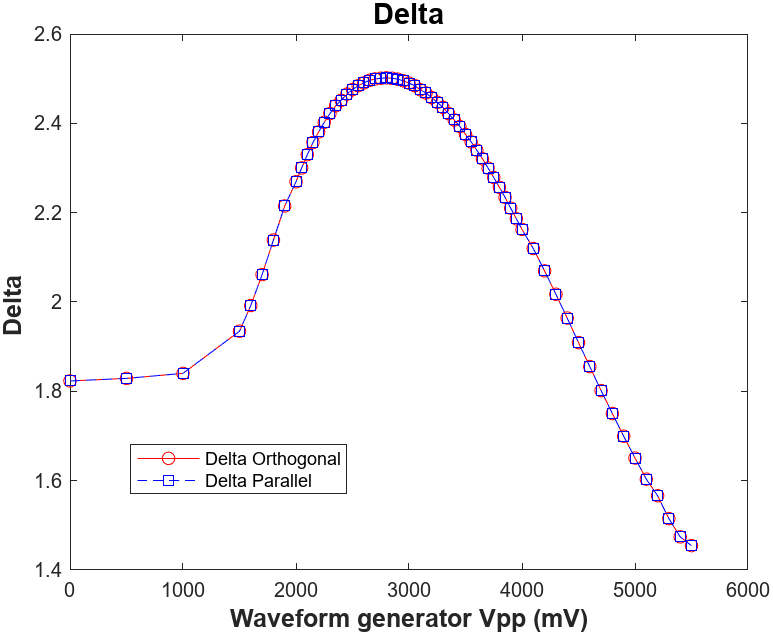
\includegraphics[width=0.6\linewidth]{figs/task34_delta.png}
    \caption{$\delta(V)$ calculated from the orthogonal and parallel configuration.}
    \label{fig:t3_4_delta}
\end{figure}

\subsection{Detection of hemozoid suspended in water}
For the detection of hemozoid suspended in water, a lock-in amplifier was employed, utilizing a lock-in frequency (20 Hz) that was twice the driving frequency (10 Hz). This approach enhances the signal-to-noise ratio, allowing for the sensitive detection of small optical signals modulated by the hemozoid. While some variability was observed in repeated measurements, the primary objective was to construct a calibration curve relating the concentration of hemozoid to the measured optical signal (Fig. \ref{fig:t6}).

% TASK 5

% The results from the lockin measurement were not very precise, and repeated mesurements yielded slightly different results. 

\begin{figure} [H]
    \centering
    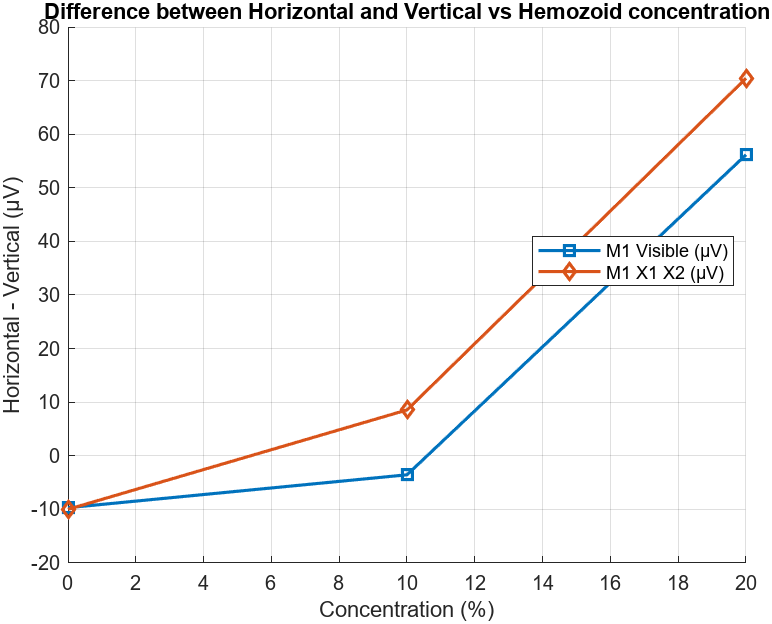
\includegraphics[width=0.6\linewidth]{figs/task6_concentration.png}
    \caption{$\delta(V)$ calculated from the orthogonal and parallel configuration.}
    \label{fig:t6}
\end{figure}

The quality of the calibration curve is limited by the few data points available. We were expecting a linear relationship (at least, for not very large concentrations where some saturation is expected), which is difficult to validate given the limited data. The discrepancy seen at the 0\% concentration sample could be accounted for by considering it the baseline effect caused by the elements other than the hemozoid. % XXX improved
Furthermore, there were more bubbles in the 0\% concentration sample. However, linear or non-linear, a well done calibration curve can be effectively used to calculate the concentration level of hemozoid by interpolation, which makes this technique useful for diagnosis.


% Conclusion
\section{Conclusion}
This laboratory exercise successfully demonstrated various principles of light polarization and its modulation using a liquid crystal cell. Key findings include the validation of Malus' Law through the characterization of film polarizers, exhibiting a clear \( \cos^2\varphi \) dependency of light intensity on analyzer orientation. The liquid crystal cell's ability to modulate light polarization was observed, with its electro-optical properties revealing a strongly non-linear response to applied voltage. Furthermore, the feasibility of detecting hemozoid in suspension through optical signal modulation was established, leading to the construction of a calibration curve.
Manually rotating the polarizer and calibrating the measurement setup introduced some limitations and errors which could be reduced by more precise automatized controls. The quality of the calibration curve for hemozoid detection was limited by the number of data points, suggesting that an increased sample size would significantly improve its linearity and predictive accuracy. Future work could focus on automating the angular adjustments and voltage controls to minimize human error and enhance measurement precision. Additionally, exploring a wider range of hemozoid concentrations and utilizing more advanced signal processing techniques could further refine the detection methodology, potentially leading to more robust diagnostic applications.

\section{Appendix}

\subsection{Revisions and Corrections from Lab Notes}
This appendix outlines significant revisions and corrections made to the experimental data analysis as initially documented in the lab notes.

- \textbf{Retardation Calculation in Tasks 3 and 4:} In the initial lab notes, the parallel (\( T_\parallel \)) and orthogonal (\( T_\perp \)) transmittances were normalized individually by their respective maximum values. This approach was incorrect for determining the retardation \( \delta \). The appropriate methodology requires normalization by the total transmittance \( T \), which can be calculated as \( T=\sqrt{T_\parallel^2+T_\perp^2} \). This correction has been implemented in the main body of this report to ensure accurate retardation values.

- \textbf{Polar Plot in Task 2:} The original lab notes for Task 2 omitted the conversion of angular measurements from degrees to radians for the polar plot. This oversight has been rectified in the current report, ensuring the correct representation of the angular dependency of light intensity.

%LLM-COMMENT: This appendix has been revised to be formal and academic.

\end{document}